\documentclass{article}
\usepackage{graphicx}
\usepackage{titling}
\usepackage{amsmath}
\usepackage{amssymb}
\usepackage{hyperref}
\usepackage{float}
\usepackage{listings}
\usepackage{booktabs}
\usepackage[table]{xcolor}
\usepackage{geometry}
\usepackage{tikz}
\usetikzlibrary{shapes.geometric, arrows, positioning, fit, calc, shadows}
\usepackage{tcolorbox}
\tcbuselibrary{skins}
\usepackage{enumitem}
\usepackage{fancyhdr}
\usepackage{pagecolor}
\usepackage{tabularx}
\usepackage{longtable}
\usepackage{array}
\usepackage{multirow}
\usepackage{microtype}
\usepackage{parskip}

% --- LIGHT MODE COLOR PALETTE ---
\definecolor{primarybg}{RGB}{255, 255, 255}
\definecolor{secondarygrey}{RGB}{80, 80, 80}
\definecolor{neutraltext}{RGB}{20, 20, 20}
\definecolor{accentblue}{RGB}{60, 170, 100}
\definecolor{accentgold}{RGB}{160, 130, 40}
\definecolor{boxbg}{RGB}{245, 247, 250}

% Setup page geometry
\geometry{a4paper, margin=0.8in, bottom=1in}

% --- GLOBAL THEME SETUP ---
\pagecolor{primarybg}
\color{neutraltext}

% Setup headers and footers
\pagestyle{fancy}
\fancyhf{}
\fancyhead[L]{\textcolor{accentblue}{\textbf{Team 5}}}
\fancyhead[C]{\textcolor{secondarygrey}{Phase 1 - Proposal \& Dataset Validation Report}}
\fancyhead[R]{}
\fancyfoot[C]{\textcolor{accentgold}{\thepage}}
\renewcommand{\headrulewidth}{1pt}
\renewcommand{\footrulewidth}{1pt}
\renewcommand{\headrule}{\hbox to\headwidth{\color{accentblue}\leaders\hrule height \headrulewidth\hfill}}
\renewcommand{\footrule}{\hbox to\headwidth{\color{accentblue}\leaders\hrule height \footrulewidth\hfill}}

% Custom box styles
\tcbset{
    mainbox/.style={
        enhanced,
        colback=boxbg,
        colframe=accentblue,
        coltext=neutraltext,
        boxrule=1pt,
        arc=3mm,
        fonttitle=\bfseries\large,
        title style={fill=accentblue, text=white},
        drop shadow={black!20!white}
    },
    quotebox/.style={
        colback=boxbg,
        colframe=accentgold,
        coltext=neutraltext,
        boxrule=0pt,
        leftrule=3mm,
        arc=2mm,
        fontupper=\itshape
    }
}

% Code-style command
\newcommand{\code}[1]{\texttt{\small #1}}

% Column types
\newcolumntype{L}[1]{>{\raggedright\arraybackslash}p{#1}}
\newcolumntype{C}[1]{>{\centering\arraybackslash}p{#1}}
\newcolumntype{R}[1]{>{\raggedleft\arraybackslash}p{#1}}

% ──────────────────────────────────────────────
\begin{document}

% --- TITLE PAGE ---
\begin{titlepage}
    \begin{center}
        \begin{minipage}[c]{0.12\textwidth}
            \includegraphics[width=\textwidth]{figures/gen/Cairo_University_Crest.png}
        \end{minipage}
        \hfill
        \begin{minipage}[c]{0.6\textwidth}
            \centering
            {\large \textbf{Cairo University - Faculty Of Engineering} \\
            Computer Engineering Department \\
            Applied Data Science Project -- Spring 2026 \par}
        \end{minipage}
        \hfill
        \begin{minipage}[c]{0.15\textwidth}
            \includegraphics[width=\textwidth]{figures/gen/cairo-no-back.png}
        \end{minipage}
    \end{center}

    \noindent{\color{accentblue}\hrulefill}

    \vspace{2cm}

    \begin{center}
        \tikz\node[draw=accentblue, line width=1mm, fill=boxbg, inner sep=1cm, rounded corners=1cm]{
            \parbox{0.8\textwidth}{
                \centering
                \vspace{0.5cm}
                {\fontsize{28}{34}\selectfont \textcolor{accentblue}{\textbf{Phase 1 - Proposal \&}} \par}
                {\fontsize{28}{34}\selectfont \textcolor{accentblue}{\textbf{Dataset Validation Report}} \par}
                \vspace{0.3cm}
                {\fontsize{22}{28}\selectfont \textcolor{accentgold}{\textbf{Team 5}} \par}
                \vspace{0.5cm}
            }
        };
    \end{center}

    \vspace{2cm}

    \begin{center}
        \begin{tcolorbox}
            \renewcommand{\arraystretch}{1.5}
            \begin{tabularx}{\textwidth}{X c c r}
                \textbf{\textcolor{accentgold}{Name}} &
                \textbf{\textcolor{accentgold}{Sec}} &
                \textbf{\textcolor{accentgold}{BN}} &
                \textbf{\textcolor{accentgold}{Email}} \\
                \midrule
                Ahmed Hamed Gaber Hamed     & \textcolor{secondarygrey}{1} & \textcolor{secondarygrey}{3}  & \textcolor{secondarygrey}{ahmed.hamed03@eng-st.cu.edu.eg} \\
                Akram Hany Karam Salam      & \textcolor{secondarygrey}{1} & \textcolor{secondarygrey}{13} & \textcolor{secondarygrey}{akram.sallam03@eng-st.cu.edu.eg} \\
                Amir Anwar Bekhit Awd Kedis & \textcolor{secondarygrey}{1} & \textcolor{secondarygrey}{14} & \textcolor{secondarygrey}{amir.awd03@eng-st.cu.edu.eg} \\
                Somia Saad Ismail El-Shemy  & \textcolor{secondarygrey}{1} & \textcolor{secondarygrey}{26} & \textcolor{secondarygrey}{somia.elshemy02@eng-st.cu.edu.eg} \\
            \end{tabularx}
        \end{tcolorbox}
    \end{center}

    \begin{center}
        \vspace{1.5cm}
        {\large \today \par}
    \end{center}

    \vfill
\end{titlepage}

\newpage
\setcounter{page}{1}
\tableofcontents
\newpage

% ════════════════════════════════════════════
\section{\textcolor{accentblue}{Abstract}}

Multi-class classification model to predict flight departure delay severity before pushback. Data sources: 2015 BTS domestic flight records (CSV) + Open-Meteo Historical Weather API. Four classes: \textbf{On Time}, \textbf{Minor Delay}, \textbf{Major Delay}, \textbf{Cancelled}. Final dataset: 116,381 rows $\times$ 55 columns. Validation found no full-row duplicates and only expected missing-value patterns.

% ════════════════════════════════════════════
\section{\textcolor{accentblue}{Problem Statement}}

\subsection*{\textcolor{accentgold}{2.1 Business Problem}}

Flight delays cause operational disruptions, increased costs, and poor passenger experience. The goal is to \textbf{predict departure delay severity before pushback}, enabling ground operations to take proportional action in advance.

\subsection*{\textcolor{accentgold}{2.2 Stakeholders}}

\textbf{Primary:} Airline operations team and airport management.

\textbf{Secondary:} Passengers and customer service teams.

\subsection*{\textcolor{accentgold}{2.3 Why Classification}}

Delay severity is a discrete outcome, not a continuous one. Each class maps to a distinct operational response, making classification the best option to use. Multi-class over binary captures severity categories. Misclassification costs are asymmetric, missing a major delay is worse than over-alerting, which is handled through business-oriented evaluation metrics.

\subsection*{\textcolor{accentgold}{2.4 Decision-Making Impact}}

\vspace{0.3em}
\begin{tcolorbox}[mainbox, title={Operational Response by Predicted Class}]
\renewcommand{\arraystretch}{1.4}
\begin{tabularx}{\textwidth}{L{2.8cm} L{3cm} X}
    \toprule
    \textbf{Predicted Class} & \textbf{Label} & \textbf{Operational Action} \\
    \midrule
    \code{on\_time}     & On Time ($\leq$15 min)   & No action \\
    \code{minor\_delay} & Minor Delay (15--45 min)  & Notify passengers, monitor connections \\
    \code{major\_delay} & Major Delay ($>$45 min)  & Rebook connections, alert ground crew \\
    \code{cancelled}    & Cancelled                 & Trigger rebooking and compensation protocols \\
    \bottomrule
\end{tabularx}
\end{tcolorbox}

\newpage
% ════════════════════════════════════════════
\section{\textcolor{accentblue}{Target Variable Definition}}

The classification target is derived from the \code{DEPARTURE\_DELAY} column (minutes) and the \code{CANCELLED} flag.

\vspace{0.3em}
\begin{tcolorbox}[mainbox, title={Class Distribution}]
\renewcommand{\arraystretch}{1.4}
\begin{tabularx}{\textwidth}{L{2.5cm} L{2.8cm} X C{1.8cm} C{1.2cm}}
    \toprule
    \textbf{Class} & \textbf{Label} & \textbf{Definition} & \textbf{Count} & \textbf{\%} \\
    \midrule
    \code{on\_time}     & On Time     & \code{DEPARTURE\_DELAY} $\leq$ 15 min (FAA standard) & 94,345 & 81.1\% \\
    \code{minor\_delay} & Minor Delay & $15 <$ \code{DEPARTURE\_DELAY} $\leq$ 45 min          & 11,433 &  9.8\% \\
    \code{major\_delay} & Major Delay & \code{DEPARTURE\_DELAY} $>$ 45 min                    &  8,833 &  7.6\% \\
    \code{cancelled}    & Cancelled   & \code{CANCELLED == 1}                                  &  1,770 &  1.5\% \\
    \bottomrule
\end{tabularx}
\end{tcolorbox}

\textbf{Why \code{DEPARTURE\_DELAY}:} The goal is pre-departure action, departure delay is the directly actionable outcome.

\textbf{Class thresholds:} The 15-minute threshold follows the FAA on-time standard. The 45-minute split is where airlines typically begin rebooking connecting passengers.

\textbf{Cancelled flights:} Retained as a distinct fourth class. They have no \code{DEPARTURE\_DELAY} but cancellation is itself a severe outcome. Final handling deferred to the preprocessing phase.

\textbf{Class imbalance:} \code{on\_time} dominates at 81.1\%. Will be addressed using \textbf{SMOTE and other techniques while training}.

% ════════════════════════════════════════════
\section{\textcolor{accentblue}{Dataset Documentation}}

\subsection*{\textcolor{accentgold}{4.1 Source 1, CSV (BTS / Kaggle)}}

\begin{tcolorbox}[mainbox, title={Dataset Overview}]
\renewcommand{\arraystretch}{1.4}
\begin{tabularx}{\textwidth}{L{3.2cm} X}
    \toprule
    \textbf{Field} & \textbf{Details} \\
    \midrule
    Name               & 2015 Flight Delays and Cancellations \\
    Provider           & US Department of Transportation, Bureau of Transportation Statistics (BTS) \\
    URL                & \href{https://www.kaggle.com/datasets/usdot/flight-delays}{\textcolor{accentblue}{\underline{kaggle.com/datasets/usdot/flight-delays}}} \\
    Citation           & U.S.\ Dept.\ of Transportation, BTS. (2015). \textit{Airline On-Time Performance Data}. Kaggle. \\
    Acquisition        & Direct CSV download (flat file) \\
    Raw Size           & $\sim$5,819,079 flight records $\times$ 31 features \\
    Sampled Size       & 116,381 rows (2\% stratified random sample by month, \code{random\_state=42}) \\
    Coverage           & All domestic US flights, calendar year 2015 \\
    License            & Public domain (US government data) \\
    \bottomrule
\end{tabularx}
\end{tcolorbox}

\vspace{0.5em}
\textbf{Key Features:}

\begin{tcolorbox}[mainbox, title={BTS Feature Descriptions}]
\renewcommand{\arraystretch}{1.3}
\begin{longtable}{L{4cm} L{1.8cm} p{7.5cm}}
    \toprule
    \textbf{Feature} & \textbf{Type} & \textbf{Description} \\
    \midrule
    \endhead
    \code{YEAR}                  & int   & Year of flight (2015) \\
    \code{MONTH}                 & int   & Month (1--12) \\
    \code{DAY}                   & int   & Day of month \\
    \code{DAY\_OF\_WEEK}         & int   & 1=Monday \ldots{} 7=Sunday \\
    \code{AIRLINE}               & str   & IATA airline carrier code (e.g., AA, DL, UA) \\
    \code{FLIGHT\_NUMBER}        & int   & Airline-assigned flight number \\
    \code{TAIL\_NUMBER}          & str   & Aircraft tail registration number \\
    \code{ORIGIN\_AIRPORT}       & str   & IATA code of departure airport \\
    \code{DESTINATION\_AIRPORT}  & str   & IATA code of arrival airport \\
    \code{SCHEDULED\_DEPARTURE}  & int   & Scheduled departure time (HHMM) \\
    \code{DEPARTURE\_TIME}       & float & Actual departure time, \textit{post-departure, excluded} \\
    \code{DEPARTURE\_DELAY}      & float & Departure delay in minutes, \textit{post-departure, excluded} \\
    \code{TAXI\_OUT}             & float & Taxi-out time in minutes, \textit{post-departure, excluded} \\
    \code{WHEELS\_OFF}           & float & Wheels-off time (HHMM), \textit{post-departure, excluded} \\
    \code{SCHEDULED\_TIME}       & float & Scheduled flight duration (minutes) \\
    \code{ELAPSED\_TIME}         & float & Actual elapsed time, \textit{post-departure, excluded} \\
    \code{AIR\_TIME}             & float & Airborne time, \textit{post-departure, excluded} \\
    \code{DISTANCE}              & int   & Flight distance (miles) \\
    \code{WHEELS\_ON}            & float & Wheels-on time, \textit{post-departure, excluded} \\
    \code{TAXI\_IN}              & float & Taxi-in time, \textit{post-departure, excluded} \\
    \code{SCHEDULED\_ARRIVAL}    & int   & Scheduled arrival time (HHMM) \\
    \code{ARRIVAL\_TIME}         & float & Actual arrival time, \textit{post-departure, excluded} \\
    \code{ARRIVAL\_DELAY}        & float & Arrival delay in minutes, used to build target label only \\
    \code{DIVERTED}              & int   & 1 if flight was diverted \\
    \code{CANCELLED}             & int   & 1 if flight was cancelled \\
    \code{CANCELLATION\_REASON}  & str   & A=Carrier, B=Weather, C=NAS, D=Security \\
    \code{AIR\_SYSTEM\_DELAY}    & float & Delay from NAS, \textit{post-departure, excluded} \\
    \code{SECURITY\_DELAY}       & float & Delay from security, \textit{post-departure, excluded} \\
    \code{AIRLINE\_DELAY}        & float & Delay from carrier, \textit{post-departure, excluded} \\
    \code{LATE\_AIRCRAFT\_DELAY} & float & Delay from late aircraft, \textit{post-departure, excluded} \\
    \code{WEATHER\_DELAY}        & float & Delay from weather, \textit{post-departure, excluded} \\
    \bottomrule
\end{longtable}
\end{tcolorbox}

\subsection*{\textcolor{accentgold}{4.2 Source 2, REST API (Open-Meteo Historical Weather)}}

\begin{tcolorbox}[mainbox, title={API Overview}]
\renewcommand{\arraystretch}{1.4}
\begin{tabularx}{\textwidth}{L{3.2cm} X}
    \toprule
    \textbf{Field} & \textbf{Details} \\
    \midrule
    Name               & Open-Meteo Historical Weather API \\
    Provider           & Open-Meteo \\
    URL                & \href{https://open-meteo.com/en/docs/historical-weather-api}{\textcolor{accentblue}{\underline{open-meteo.com/en/docs/historical-weather-api}}} \\
    Cost               & Free, no API key required \\
    Acquisition        & HTTP GET requests, one call per unique airport per year, cached as JSON in \code{data/raw/weather\_cache/\{IATA\}\_\{YEAR\}.json} \\
    Query Parameters   & \code{latitude}, \code{longitude}, \code{start\_date=2015-01-01}, \code{end\_date=2015-12-31}, \code{hourly} variables, \code{timezone=America/New\_York} \\
    \bottomrule
\end{tabularx}
\end{tcolorbox}

\vspace{0.5em}
\textbf{11 Weather Variables Retrieved (per airport, per hour):}

\begin{tcolorbox}[mainbox, title={Weather Feature Descriptions}]
\renewcommand{\arraystretch}{1.3}
\begin{tabularx}{\textwidth}{L{3.8cm} L{3.8cm} L{1.4cm} X}
    \toprule
    \textbf{Feature (origin)} & \textbf{Feature (dest)} & \textbf{Unit} & \textbf{Description} \\
    \midrule
    \code{temperature\_c}          & \code{dest\_temperature\_c}          & °C   & Air temperature at 2\,m \\
    \code{precipitation\_mm}       & \code{dest\_precipitation\_mm}       & mm   & Total precipitation \\
    \code{rain\_mm}                & \code{dest\_rain\_mm}                & mm   & Rain component \\
    \code{snowfall\_cm}            & \code{dest\_snowfall\_cm}            & cm   & Snowfall \\
    \code{wind\_speed\_kmh}        & \code{dest\_wind\_speed\_kmh}        & km/h & Wind speed at 10\,m \\
    \code{wind\_direction\_deg}    & \code{dest\_wind\_direction\_deg}    & deg  & Wind direction \\
    \code{wind\_gusts\_kmh}        & \code{dest\_wind\_gusts\_kmh}        & km/h & Wind gusts \\
    \code{cloud\_cover\_pct}       & \code{dest\_cloud\_cover\_pct}       & \%   & Cloud cover \\
    \code{weather\_code}           & \code{dest\_weather\_code}           & WMO  & Precipitation/fog/storm type \\
    \code{relative\_humidity\_pct} & \code{dest\_relative\_humidity\_pct} & \%   & Relative humidity \\
    \code{pressure\_msl\_hpa}      & \code{dest\_pressure\_msl\_hpa}      & hPa  & Sea-level pressure \\
    \bottomrule
\end{tabularx}
\end{tcolorbox}

\begin{tcolorbox}[quotebox]
\textbf{Why destination weather?} Destination weather at scheduled arrival time is knowable before departure (weather forecasts) and directly influences whether the plane can land. Including it improves the model's ability to predict arrival delays caused by destination-side conditions.
\end{tcolorbox}


\newpage
% ════════════════════════════════════════════
\section{\textcolor{accentblue}{Merge Strategy}}

\textbf{Type:} Horizontal merge, weather columns are appended to each flight row.

\vspace{0.3em}
\begin{tcolorbox}[mainbox, title={Join Keys}]
\renewcommand{\arraystretch}{1.4}
\begin{tabularx}{\textwidth}{L{3cm} X L{4.5cm}}
    \toprule
    \textbf{Join} & \textbf{Key} & \textbf{Weather Columns Added} \\
    \midrule
    Origin weather      & \code{(ORIGIN\_AIRPORT, MONTH, DAY, departure\_hour)}                    & 11 cols (\code{temperature\_c}, \ldots) \\
    Destination weather & \code{(DESTINATION\_AIRPORT, MONTH, arrival\_day, scheduled\_arrival\_hour)} & 11 cols (\code{dest\_temperature\_c}, \ldots) \\
    \bottomrule
\end{tabularx}
\end{tcolorbox}

\textbf{Timezone handling:} The Open-Meteo API returns timestamps in \code{America/New\_York}. Flight schedules are in each airport's local time. \code{timezonefinder} resolves each airport's IANA timezone from its coordinates, \code{zoneinfo} converts local departure/arrival hours to Eastern before building the lookup key, correctly handling DST for all 2015 dates.

\textbf{Overnight flights:} Arrival day is computed by adding \code{SCHEDULED\_TIME} (minutes) to departure hour, detecting day rollovers where the flight arrives the next calendar day.

\vspace{0.3em}
\begin{tcolorbox}[mainbox, title={Row Counts Before/After Merging}]
\renewcommand{\arraystretch}{1.4}
\begin{tabularx}{\textwidth}{X R{3.5cm}}
    \toprule
    \textbf{Stage} & \textbf{Row Count} \\
    \midrule
    Raw BTS flights CSV                                           & $\sim$5,819,079 \\
    After 2\% stratified sample (by month)                        & 116,381 \\
    After weather join (no rows dropped)                          & 116,381 \\
    Rows with missing origin weather (numeric airport codes)       & 9,837 \enspace(8.45\%) \\
    Rows with missing destination weather (numeric airport codes)  & 9,823 \enspace(8.44\%) \\
    \textbf{Final dataset}                                        & \textbf{116,381 $\times$ 55 cols} \\
    \bottomrule
\end{tabularx}
\end{tcolorbox}

\begin{tcolorbox}[quotebox]
The join does not drop rows, flights with no valid airport code get \code{NaN} weather values. These $\sim$9,837 rows will be dropped in the cleaning phase as weather is a core feature set.
\end{tcolorbox}

% ════════════════════════════════════════════
\section{\textcolor{accentblue}{Engineered Features}}

Features derived during acquisition (present in \code{flights\_weather.csv}):

\begin{tcolorbox}[mainbox, title={Acquired Engineered Features}]
\renewcommand{\arraystretch}{1.4}
\begin{tabularx}{\textwidth}{L{4cm} L{5.5cm} X}
    \toprule
    \textbf{Feature} & \textbf{Derivation} & \textbf{Notes} \\
    \midrule
    \code{departure\_hour}          & \code{SCHEDULED\_DEPARTURE // 100}  & Hour of scheduled departure (0--23) \\
    \code{scheduled\_arrival\_hour} & \code{SCHEDULED\_ARRIVAL // 100}    & Hour of scheduled arrival (0--23) \\
    \code{dest\_*} weather columns  & Open-Meteo API at destination       & 11 destination weather features \\
    \bottomrule
\end{tabularx}
\end{tcolorbox}

Additional features to be engineered during the preprocessing phase:

\begin{itemize}[label=\textcolor{accentblue}{\textbullet}]
    \item \code{is\_weekend}, \code{is\_holiday}
    \item \code{route} (ORIGIN + DESTINATION)
    \item Historical delay rates per airline/route
    \item \code{busy\_bad\_weather\_score}
\end{itemize}

% ════════════════════════════════════════════
\section{\textcolor{accentblue}{Data Validation Report}}

Validation was performed via \code{src/validation/validate.py} covering 12 checks. Results are reproduced from \code{notebooks/validation\_report.ipynb}.

\begin{tcolorbox}[quotebox]
\textbf{Dataset:} \code{data/processed/flights\_weather.csv}, 116,381 rows $\times$ 55 columns
\end{tcolorbox}

\subsection*{\textcolor{accentgold}{7.1 Summary}}

\begin{tcolorbox}[mainbox, title={Validation Checks Summary}]
\renewcommand{\arraystretch}{1.4}
\begin{tabularx}{\textwidth}{L{4cm} X}
    \toprule
    \textbf{Check} & \textbf{Result} \\
    \midrule
    Schema             & All 55 columns present, all types are correct \\
    Completeness       & Weather cols 8.45\% null (numeric airports, expected), delay breakdown 81.75\% null (expected, only set when delayed), \code{TAIL\_NUMBER} 0.22\% null \\
    Duplicates         & 0 full-row duplicates, 864 flight-level duplicates (codeshares, expected) \\
    Value Ranges       & All numeric values within expected bounds \\
    Consistency        & 97 cancelled flights have a \code{DEPARTURE\_TIME} (taxied before cancellation) \\
    Outliers           & Detected via IQR, delay and distance columns show expected right-skewed extremes \\
    Referential Integrity & 9,723 rows use numeric FAA IDs instead of IATA codes, no coordinate match \\
    Format Validation  & All IATA codes, HHMM times, and YEAR values conform to expected formats \\
    Temporal Validity  & All (MONTH, DAY) combinations are valid calendar dates \\
    Cardinality        & 14 unique airlines, $\sim$322 unique origin and destination airports \\
    Statistics         & Descriptive statistics within expected bounds for all numeric columns \\
    Target Readiness   & 340 non-cancelled rows unlabellable (no \code{ARRIVAL\_DELAY}), 4-class distribution documented \\
    \bottomrule
\end{tabularx}
\end{tcolorbox}

\subsection*{\textcolor{accentgold}{7.2 Completeness, Missing Values}}

\begin{tcolorbox}[mainbox, title={Missing Value Analysis}]
\renewcommand{\arraystretch}{1.3}
\begin{tabularx}{\textwidth}{X C{2.2cm} C{1.8cm} L{3.5cm}}
    \toprule
    \textbf{Column} & \textbf{Missing Count} & \textbf{Missing \%} & \textbf{Explanation} \\
    \midrule
    \code{CANCELLATION\_REASON}                              & 114,611 & 98.48\% & Cancelled flights only, expected \\
    \code{LATE\_AIRCRAFT\_DELAY}                             &  95,143 & 81.75\% & Delayed flights only, expected \\
    \code{AIR\_SYSTEM\_DELAY}                                &  95,143 & 81.75\% & Same, expected \\
    \code{SECURITY\_DELAY}                                   &  95,143 & 81.75\% & Same, expected \\
    \code{WEATHER\_DELAY}                                    &  95,143 & 81.75\% & Same, expected \\
    \code{AIRLINE\_DELAY}                                    &  95,143 & 81.75\% & Same, expected \\
    Origin weather cols (11)                                  &   9,837 &  8.45\% & Numeric airport codes, no IATA match \\
    Dest weather cols (11)                                    &   9,823 &  8.44\% & Same (slightly different set) \\
    \code{ARRIVAL\_DELAY}                                    &   2,110 &  1.81\% & Cancelled + 340 diverted, expected \\
    \code{AIR\_TIME} / \code{ELAPSED\_TIME}                  &   2,110 &  1.81\% & Cancelled/diverted, expected \\
    \code{TAXI\_IN} / \code{WHEELS\_ON} / \code{ARRIVAL\_TIME} & 1,829 &  1.57\% & Flights that did not arrive \\
    \code{WHEELS\_OFF} / \code{TAXI\_OUT}                    &   1,748 &  1.50\% & Flights that did not depart \\
    \code{DEPARTURE\_TIME} / \code{DEPARTURE\_DELAY}         &   1,673 &  1.44\% & Cancelled flights \\
    \code{TAIL\_NUMBER}                                      &     258 &  0.22\% & Missing tail registration \\
    \bottomrule
\end{tabularx}
\end{tcolorbox}

\subsection*{\textcolor{accentgold}{7.3 Duplicates}}

\begin{tcolorbox}[mainbox, title={Duplicate Check}]
\renewcommand{\arraystretch}{1.4}
\begin{tabularx}{\textwidth}{X C{1.8cm} L{6cm}}
    \toprule
    \textbf{Check} & \textbf{Count} & \textbf{Notes} \\
    \midrule
    Full-row duplicates & 0 & No exact row duplicates \\
    Flight-level duplicates (\code{AIRLINE + FLIGHT\_NUMBER + MONTH + DAY}) & 864 & Codeshare flights, multiple airlines operating same physical flight, expected \\
    \bottomrule
\end{tabularx}
\end{tcolorbox}

\subsection*{\textcolor{accentgold}{7.4 Value Ranges}}

\begin{tcolorbox}[mainbox, title={Numeric Column Range Checks}]
\renewcommand{\arraystretch}{1.4}
\begin{tabularx}{\textwidth}{L{5cm} L{3cm} C{2.5cm}}
    \toprule
    \textbf{Column} & \textbf{Valid Range} & \textbf{Violations} \\
    \midrule
    \code{MONTH}                & 1--12   & 0 \\
    \code{DAY}                  & 1--31   & 0 \\
    \code{DAY\_OF\_WEEK}        & 1--7    & 0 \\
    \code{SCHEDULED\_DEPARTURE} & 0--2359 & 0 \\
    \code{DISTANCE}             & $>0$    & 0 \\
    \code{SCHEDULED\_TIME}      & $>0$    & 0 \\
    \bottomrule
\end{tabularx}
\end{tcolorbox}

\begin{tcolorbox}[quotebox]
$\sim$9,837 rows have numeric values in \code{ORIGIN\_AIRPORT} (e.g., \code{14747}) that are FAA numeric station IDs rather than IATA codes. These are not range violations, they are a data quality issue documented under Referential Integrity.
\end{tcolorbox}

\subsection*{\textcolor{accentgold}{7.5 Consistency Checks}}

\begin{tcolorbox}[mainbox, title={Consistency Results}]
\renewcommand{\arraystretch}{1.4}
\begin{tabularx}{\textwidth}{X C{2.2cm} L{5.5cm}}
    \toprule
    \textbf{Check} & \textbf{Rows Affected} & \textbf{Description} \\
    \midrule
    Canceled flights with \code{DEPARTURE\_TIME} & 97 & Flights that was canceled while on ground before they took off (due to any issues) \\
    \bottomrule
\end{tabularx}
\end{tcolorbox}
\newpage
\subsection*{\textcolor{accentgold}{7.6 Outlier Detection (IQR Method, 1.5$\times$ Fence)}}

Outliers were detected using the IQR method across key numeric columns. Extreme values in delay-related columns are expected (heavy weather events, ground stops) and will be handled during the cleaning phase by binning rather than dropping.

\begin{figure}[ht]
    \centering
    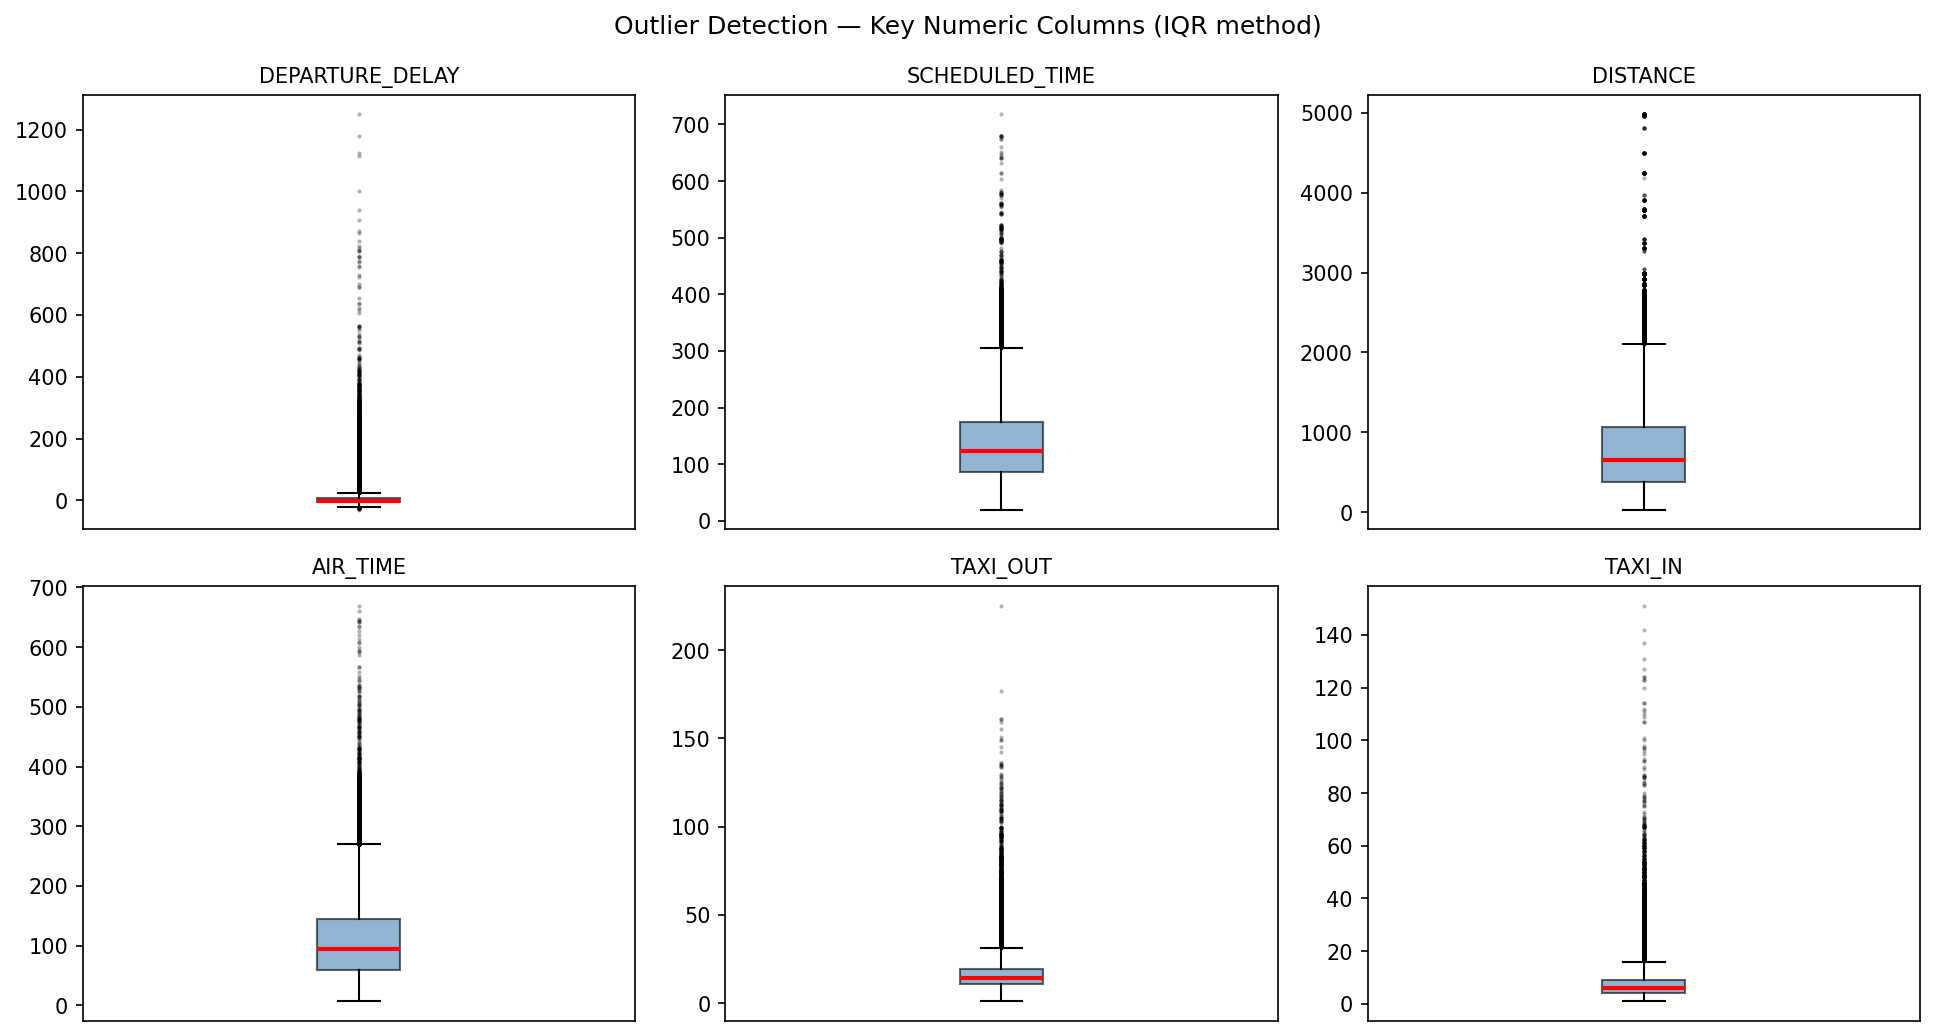
\includegraphics[width=1\textwidth]{figures/eda/outlier_boxplots.png}
    \caption{Outliers using IQR method}
    \label{fig:my_label}
\end{figure}


\subsection*{\textcolor{accentgold}{7.7 Referential Integrity}}

\begin{tcolorbox}[mainbox, title={Referential Integrity Checks}]
\renewcommand{\arraystretch}{1.4}
\begin{tabularx}{\textwidth}{X C{2.5cm} L{4.5cm}}
    \toprule
    \textbf{Check} & \textbf{Unmatched Count} & \textbf{Unmatched Values (sample)} \\
    \midrule
    \code{AIRLINE} codes vs \code{airlines.csv}   & 0     & All match \\
    IATA airport codes vs \code{airports.csv}      & 9,723 & Numeric FAA IDs (e.g., 14747, 13830), no IATA equivalent \\
    \bottomrule
\end{tabularx}
\end{tcolorbox}

The 9,723 rows with numeric airport codes ($\sim$8.35\% of the dataset) have no coordinates and therefore no weather data. \textbf{Decision:} drop in the cleaning phase, weather is a core feature set and imputation would be meaningless.

\subsection*{\textcolor{accentgold}{7.8 Format Validation}}

\begin{tcolorbox}[mainbox, title={Format Checks}]
\renewcommand{\arraystretch}{1.4}
\begin{tabularx}{\textwidth}{X C{3cm}}
    \toprule
    \textbf{Check} & \textbf{Violations} \\
    \midrule
    IATA codes (3 uppercase letters)               & 0 (among non-numeric codes) \\
    HHMM times (minutes 00--59)                    & 0 \\
    \code{YEAR} = 2015                             & 0 \\
    \code{CANCELLATION\_REASON} in \{A, B, C, D\}  & 0 \\
    \bottomrule
\end{tabularx}
\end{tcolorbox}

\subsection*{\textcolor{accentgold}{7.9 Temporal Validity}}

All (MONTH, DAY) combinations are valid calendar dates for 2015. No invalid dates detected.

\subsection*{\textcolor{accentgold}{7.10 Cardinality}}

\begin{tcolorbox}[mainbox, title={Cardinality Summary}]
\renewcommand{\arraystretch}{1.4}
\begin{tabularx}{\textwidth}{L{5cm} C{2.5cm} X}
    \toprule
    \textbf{Column} & \textbf{Unique Values} & \textbf{Top Values} \\
    \midrule
    \code{AIRLINE}              & 14        & WN, DL, AA, UA, OO \\
    \code{ORIGIN\_AIRPORT}      & $\sim$322 & ATL, ORD, DFW, LAX, DEN \\
    \code{DESTINATION\_AIRPORT} & $\sim$322 & ATL, ORD, DFW, LAX, DEN \\
    \code{DAY\_OF\_WEEK}        & 7         &, \\
    \code{CANCELLATION\_REASON} & 4         & B (Weather), A (Carrier), C (NAS), D (Security) \\
    \bottomrule
\end{tabularx}
\end{tcolorbox}

\subsection*{\textcolor{accentgold}{7.11 Target Variable Readiness}}

\begin{tcolorbox}[mainbox, title={Target Readiness Metrics}]
\renewcommand{\arraystretch}{1.4}
\begin{tabularx}{\textwidth}{X C{3.5cm}}
    \toprule
    \textbf{Metric} & \textbf{Value} \\
    \midrule
    Total rows                           & 116,381 \\
    Cancelled flights                    & 1,770 \\
    \code{DEPARTURE\_DELAY} nulls (non-cancelled) & 0 \\
    Unlabellable rows                    & 0 \\
    Labellable rows                      & 116,381 \\
    \bottomrule
\end{tabularx}
\end{tcolorbox}

\vspace{0.3em}
\textbf{Class distribution (target: \code{DEPARTURE\_DELAY}):}

\begin{tcolorbox}[mainbox, title={Final Class Distribution}]
\renewcommand{\arraystretch}{1.4}
\begin{tabularx}{\textwidth}{L{3cm} L{3.5cm} X C{1.5cm}}
    \toprule
    \textbf{Class} & \textbf{Label} & \textbf{Count} & \textbf{\%} \\
    \midrule
    \code{on\_time}     & On Time ($\leq$15 min)   & 94,345 & 81.1\% \\
    \code{minor\_delay} & Minor Delay (15--45 min)  & 11,433 &  9.8\% \\
    \code{major\_delay} & Major Delay ($>$45 min)  &  8,833 &  7.6\% \\
    \code{cancelled}    & Cancelled                 &  1,770 &  1.5\% \\
    \bottomrule
\end{tabularx}
\end{tcolorbox}

\begin{figure}[ht]
    \centering
    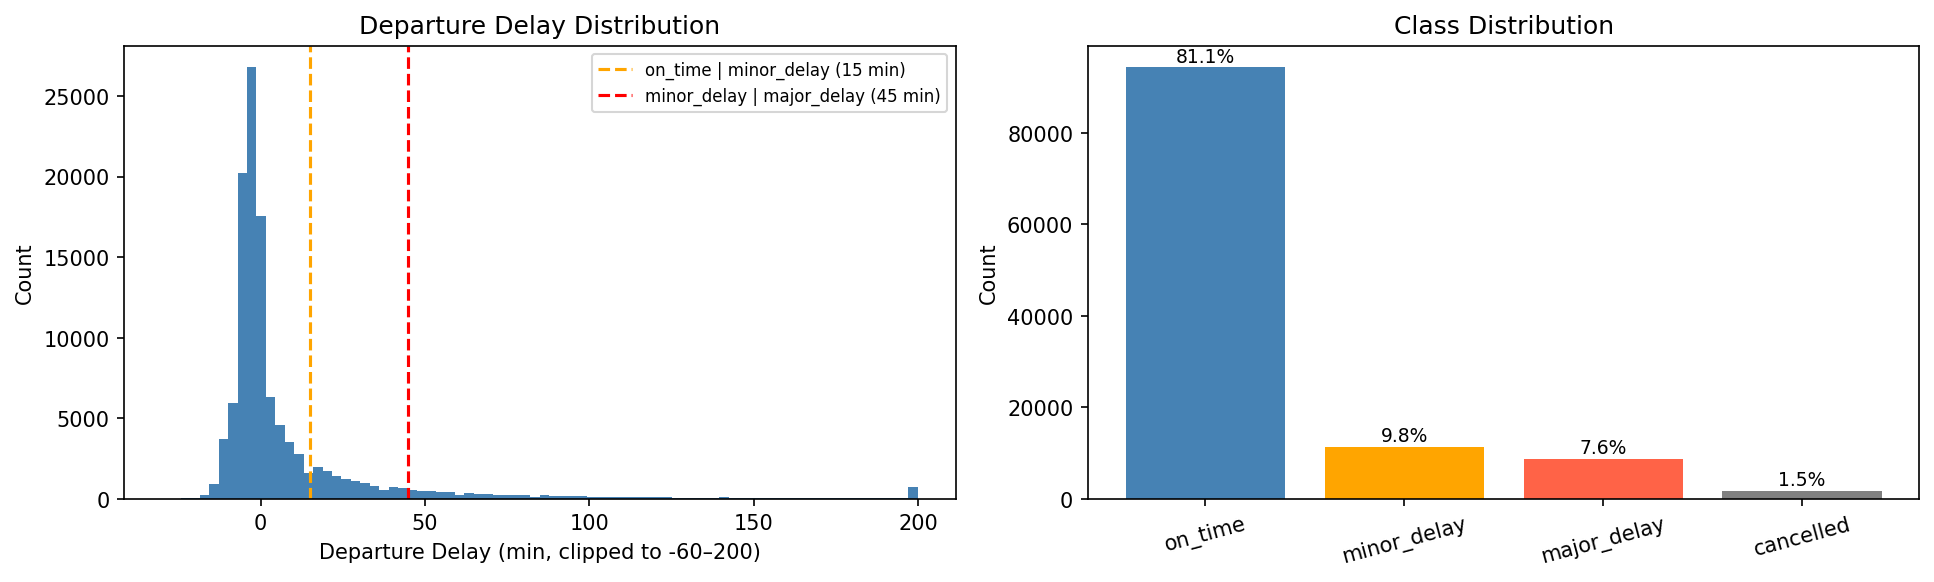
\includegraphics[width=1\textwidth]{figures/eda/target_readiness.png}
    \caption{Departure Delay Classes}
    \label{fig:my_label}
\end{figure}

\subsection*{\textcolor{accentgold}{7.12 Known Issues and Planned Resolutions}}

\begin{tcolorbox}[mainbox, title={Known Issues}]
\renewcommand{\arraystretch}{1.4}
\begin{tabularx}{\textwidth}{X C{1.8cm} C{1.8cm} L{4.2cm}}
    \toprule
    \textbf{Issue} & \textbf{Count} & \textbf{Severity} & \textbf{Planned Resolution} \\
    \midrule
    Rows with numeric airport codes (no weather)          & 9,723  & Medium & Drop in cleaning phase \\
    Cancelled flights with \code{DEPARTURE\_TIME}         & 97     & Low    & Document as data quirk, keep \\
    Missing \code{TAIL\_NUMBER}                           & 258    & Low    & Drop column, not a model feature \\
    Delay breakdown cols (post-departure leakage)          & 5 cols & High   & Drop columns in cleaning phase \\
    \bottomrule
\end{tabularx}
\end{tcolorbox}

% ════════════════════════════════════════════
\section{\textcolor{accentblue}{Preprocessing, Transformation \& Engineering}}

\textit{Placeholder: add preprocessing, transformation, and feature engineering content here.}

% ════════════════════════════════════════════
\section{\textcolor{accentblue}{Exploratory Data Analysis (EDA)}}

\textit{Placeholder: add EDA content here.}

% ════════════════════════════════════════════
\section{\textcolor{accentblue}{Model Development}}

\textit{Placeholder: add model development content here.}

% ════════════════════════════════════════════
\section{\textcolor{accentblue}{Experiment Tracking with MLflow}}

\textit{Placeholder: add MLflow experiment tracking content here.}

% ════════════════════════════════════════════
\section{\textcolor{accentblue}{Testing}}

\textit{Placeholder: add testing content here.}

% ════════════════════════════════════════════
\section{\textcolor{accentblue}{Results \& Evaluation}}

\textit{Placeholder: add results and evaluation content here.}

% ════════════════════════════════════════════
\section{\textcolor{accentblue}{Code Automation}}

\textit{Placeholder: add code automation content here.}

% ════════════════════════════════════════════
\section{\textcolor{accentblue}{Continuous Integration}}

\textit{Placeholder: add continuous integration content here.}

% ════════════════════════════════════════════
\section{\textcolor{accentblue}{Limitations \& Future Work}}

\textit{Placeholder: add limitations and future work content here.}

% ════════════════════════════════════════════
\section{\textcolor{accentblue}{Team Contributions}}

\textit{Placeholder: add team contributions content here.}

\end{document}